%----------------------------------------------------------------------------------------
\begin{frame}
\frametitle{L'identité numérique c'est quoi?}


\begin{block}{Définition}
\begin{itemize}
\justifying{
\item L'identité numérique, c'est l'ensemble des données publiques que l'on peut trouver sur Internet et rattacher à une personne, en l'occurence moi.
\item C'est la fameuse e-reputation.
}
\end{itemize}
\end{block}

\end{frame}

%----------------------------------------------------------------------------------------
\begin{frame}
\frametitle{L'image que je donne de moi}

\justifying{
\begin{block}{Googler "son nom".}
\begin{itemize}
\item Les résultats apparaissant sont-ils bien ce que l'on souhaite?
\end{itemize}
\end{block}
}
\begin{center}
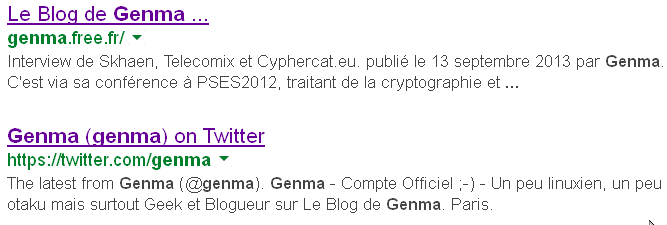
\includegraphics[scale=0.3] {./materials/Google01.png}
\\
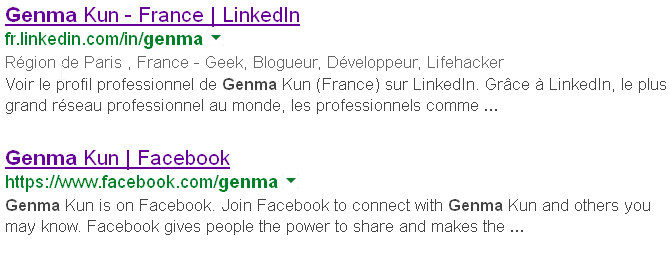
\includegraphics[scale=0.3] {./materials/Google02.png}
\end{center}

\end{frame}

%----------------------------------------------------------------------------------------
\begin{frame}
\frametitle{Adage}


\begin{block}{Les paroles s'envolent, les écrits restent}
\begin{itemize}
\justifying{
\item Cet adage est encore plus vrai avec Internet.
\item  Il faut partir du principe que ce que l'on dit sera toujours accessible, même des années après.
\item Tout ce qui est sur Internet est public ou le sera (même si c'est "privé". Les conditions d'utilisation évoulent. Cf.Facebook).
\item Il ne faut donc pas abuser de la liberté d'expression et rester respectueux des lois en vigueurs.
}
\end{itemize}
\end{block}


\end{frame}

%----------------------------------------------------------------------------------------
\begin{frame}
\frametitle{Le pseudonymat}


\begin{block}{Défintions}
\begin{itemize}
\justifying{
\item Contraction des termes pseudonyme et anonymat, le terme de pseudonymat reflète assez bien la volonté contradictoire d’être un personnage publique et de rester anonyme...
\item Avoir un pseudonyme ne veut pas dire faire et dire n'importe quoi.
\item Il en va de l'image que je renvoie, que je donne de moi et de ma crédibilité présente et à venir.
\item Un pseudonyme, c'est aussi une identité publique, qui est associée à un ensemble cohérent de compte qui forme un tout : mon blog, mon Twitter, mon compte Facebook.
\item L'identité numérique est l'ensemble des données publiques associées à cette identité. 
}
\end{itemize}
\end{block}

\end{frame}


%----------------------------------------------------------------------------------------
\begin{frame}
\frametitle{Exemples}

\begin{block}{Twitter}
\begin{center}
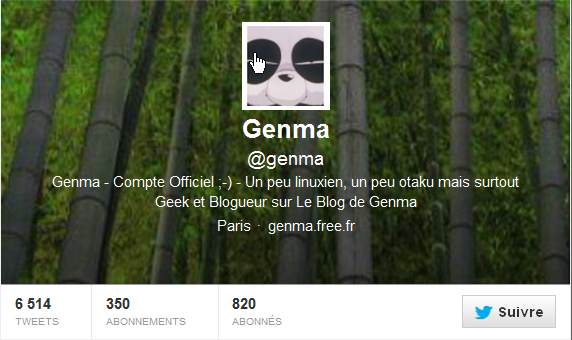
\includegraphics[scale=0.3] {./materials/Twitter.png}
\end{center}
\end{block}

\begin{block}{Linkedin}
\begin{center}
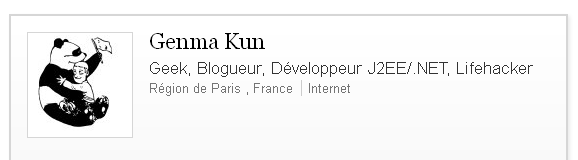
\includegraphics[scale=0.3] {./materials/Linkedin.png}
\end{center}
\end{block}

\end{frame}

